\chapter{Assignment 8}\label{ass8}

\section{Task 1}\label{ass8_t1}

The following graphs will each represent one iteration of the hard A* variation on the given graph.\\
The green circles are nodes in the open list, red ones are in the closed list and the blue ones are unknown.

\noindent And the green numbers aside from the nodes are the original heuristic estimates, while the red numbers are the updated costs to reach that node and the red letter is the predecessor.

\definecolor {processblue}{cmyk}{0.96,0,0,0}
\definecolor {processred}{cmyk}{0,0.96,0,0}
\definecolor {processgreen}{cmyk}{0.96,0,0.96,0}
\tikzset{every label/.style={green}}
\tikzset{closed/.style={ circle ,top color =white , bottom color = processred!60 ,
draw,processred , text=blue , minimum width =1 cm}}
\tikzset{open/.style={ circle ,top color =white , bottom color = processgreen!60 ,
draw,processgreen , text=blue , minimum width =1 cm}}
\tikzset{state/.style ={ circle ,top color =white , bottom color = processblue!60 ,
draw,processblue , text=blue , minimum width =1 cm}}
\begin {center}
  \begin {tikzpicture}[- ,auto ,node distance = 2 cm and 3cm ,on grid ,
  semithick]
    \node[open,label={below:\small 19 \textcolor{red}{0}}] (H){h};
    \node[state,label={below:\small 1}] (G) [left = of H] {g};
    \node[state,label={below:\small 20}] (E) [right = of H] {e};
    \node[state,label={\small 42}] (C) [above right = of H] {c};
    \node[state,label={right:\small 35}] (D) [above left = of H] {d};
    \node[state,label={\small 0}] (A) [above left = of C] {a};
    \node[state,label={\small 9}] (B) [left = of D] {b};
    \node[state,label={below:\small 18}] (F) [left = of G] {f};
    \path (H) edge [left] node[below =0.15 cm] {10} (G);
    \path (H) edge [right] node[below =0.15 cm] {10} (E);
    \path (H) edge [left] node[above] {10} (C);
    \path (H) edge [left] node[below =0.15 cm] {10} (D);
    \path (E) edge [left] node[left =0.15 cm] {10} (C);
    \path (C) edge [left] node[below =0.15 cm] {10} (A);
    \path (G) edge [left] node[left =0.15 cm] {10} (D);
    \path (D) edge [left] node[below =0.15 cm] {10} (A);
    \path (D) edge [left] node[below =0.15 cm] {10} (B);
    \path (G) edge [left] node[below =0.15 cm] {10} (F);
    \path (F) edge [right] node[left =0.15 cm] {10} (B);
    \path (B) edge [left] node[above =0.15 cm] {10} (A);
  \end{tikzpicture}
\end{center}

\begin {center}
  \begin {tikzpicture}[- ,auto ,node distance = 2 cm and 3cm ,on grid ,
  semithick]
    \node[closed,label={below:\small 19 \textcolor{red}{0}}] (H){h};
    \node[open,label={below:\small 1 \textcolor{red}{11 h}}] (G) [left = of H] {g};
    \node[open,label={below:\small 20 \textcolor{red}{30 h}}] (E) [right = of H] {e};
    \node[open,label={\small 42 \textcolor{red}{52 h}}] (C) [above right = of H] {c};
    \node[open,label={right:\small 35 \textcolor{red}{45 h}}] (D) [above left = of H] {d};
    \node[state,label={\small 0}] (A) [above left = of C] {a};
    \node[state,label={\small 9}] (B) [left = of D] {b};
    \node[state,label={below:\small 18}] (F) [left = of G] {f};
    \path (H) edge [left] node[below =0.15 cm] {10} (G);
    \path (H) edge [right] node[below =0.15 cm] {10} (E);
    \path (H) edge [left] node[above] {10} (C);
    \path (H) edge [left] node[below =0.15 cm] {10} (D);
    \path (E) edge [left] node[left =0.15 cm] {10} (C);
    \path (C) edge [left] node[below =0.15 cm] {10} (A);
    \path (G) edge [left] node[left =0.15 cm] {10} (D);
    \path (D) edge [left] node[below =0.15 cm] {10} (A);
    \path (D) edge [left] node[below =0.15 cm] {10} (B);
    \path (G) edge [left] node[below =0.15 cm] {10} (F);
    \path (F) edge [right] node[left =0.15 cm] {10} (B);
    \path (B) edge [left] node[above =0.15 cm] {10} (A);
  \end{tikzpicture}
\end{center}

\begin {center}
  \begin {tikzpicture}[- ,auto ,node distance = 2 cm and 3cm ,on grid ,
  semithick]
    \node[closed,label={below:\small 19 \textcolor{red}{0}}] (H){h};
    \node[closed,label={below:\small 1 \textcolor{red}{11 h}}] (G) [left = of H] {g};
    \node[open,label={below:\small 20 \textcolor{red}{30 h}}] (E) [right = of H] {e};
    \node[open,label={\small 42 \textcolor{red}{52 h}}] (C) [above right = of H] {c};
    \node[open,label={right:\small 35 \textcolor{red}{45 h}}] (D) [above left = of H] {d};
    \node[state,label={\small 0}] (A) [above left = of C] {a};
    \node[state,label={\small 9}] (B) [left = of D] {b};
    \node[open,label={below:\small 18 \textcolor{red}{38 g}}] (F) [left = of G] {f};
    \path (H) edge [left] node[below =0.15 cm] {10} (G);
    \path (H) edge [right] node[below =0.15 cm] {10} (E);
    \path (H) edge [left] node[above] {10} (C);
    \path (H) edge [left] node[below =0.15 cm] {10} (D);
    \path (E) edge [left] node[left =0.15 cm] {10} (C);
    \path (C) edge [left] node[below =0.15 cm] {10} (A);
    \path (G) edge [left] node[left =0.15 cm] {10} (D);
    \path (D) edge [left] node[below =0.15 cm] {10} (A);
    \path (D) edge [left] node[below =0.15 cm] {10} (B);
    \path (G) edge [left] node[below =0.15 cm] {10} (F);
    \path (F) edge [right] node[left =0.15 cm] {10} (B);
    \path (B) edge [left] node[above =0.15 cm] {10} (A);
  \end{tikzpicture}
\end{center}

\begin {center}
  \begin {tikzpicture}[- ,auto ,node distance = 2 cm and 3cm ,on grid ,
  semithick]
    \node[closed,label={below:\small 19 \textcolor{red}{0}}] (H){h};
    \node[closed,label={below:\small 1 \textcolor{red}{11 h}}] (G) [left = of H] {g};
    \node[closed,label={below:\small 20 \textcolor{red}{30 h}}] (E) [right = of H] {e};
    \node[open,label={\small 42 \textcolor{red}{52 h}}] (C) [above right = of H] {c};
    \node[open,label={right:\small 35 \textcolor{red}{45 h}}] (D) [above left = of H] {d};
    \node[state,label={\small 0}] (A) [above left = of C] {a};
    \node[state,label={\small 9}] (B) [left = of D] {b};
    \node[open,label={below:\small 18 \textcolor{red}{38 g}}] (F) [left = of G] {f};
    \path (H) edge [left] node[below =0.15 cm] {10} (G);
    \path (H) edge [right] node[below =0.15 cm] {10} (E);
    \path (H) edge [left] node[above] {10} (C);
    \path (H) edge [left] node[below =0.15 cm] {10} (D);
    \path (E) edge [left] node[left =0.15 cm] {10} (C);
    \path (C) edge [left] node[below =0.15 cm] {10} (A);
    \path (G) edge [left] node[left =0.15 cm] {10} (D);
    \path (D) edge [left] node[below =0.15 cm] {10} (A);
    \path (D) edge [left] node[below =0.15 cm] {10} (B);
    \path (G) edge [left] node[below =0.15 cm] {10} (F);
    \path (F) edge [right] node[left =0.15 cm] {10} (B);
    \path (B) edge [left] node[above =0.15 cm] {10} (A);
  \end{tikzpicture}
\end{center}

\begin {center}
  \begin {tikzpicture}[- ,auto ,node distance = 2 cm and 3cm ,on grid ,
  semithick]
    \node[closed,label={below:\small 19 \textcolor{red}{0}}] (H){h};
    \node[closed,label={below:\small 1 \textcolor{red}{11 h}}] (G) [left = of H] {g};
    \node[closed,label={below:\small 20 \textcolor{red}{30 h}}] (E) [right = of H] {e};
    \node[open,label={\small 42 \textcolor{red}{52 h}}] (C) [above right = of H] {c};
    \node[open,label={right:\small 35 \textcolor{red}{45 h}}] (D) [above left = of H] {d};
    \node[state,label={\small 0}] (A) [above left = of C] {a};
    \node[open,label={\small 9 \textcolor{red}{39 f}}] (B) [left = of D] {b};
    \node[closed,label={below:\small 18 \textcolor{red}{38 g}}] (F) [left = of G] {f};
    \path (H) edge [left] node[below =0.15 cm] {10} (G);
    \path (H) edge [right] node[below =0.15 cm] {10} (E);
    \path (H) edge [left] node[above] {10} (C);
    \path (H) edge [left] node[below =0.15 cm] {10} (D);
    \path (E) edge [left] node[left =0.15 cm] {10} (C);
    \path (C) edge [left] node[below =0.15 cm] {10} (A);
    \path (G) edge [left] node[left =0.15 cm] {10} (D);
    \path (D) edge [left] node[below =0.15 cm] {10} (A);
    \path (D) edge [left] node[below =0.15 cm] {10} (B);
    \path (G) edge [left] node[below =0.15 cm] {10} (F);
    \path (F) edge [right] node[left =0.15 cm] {10} (B);
    \path (B) edge [left] node[above =0.15 cm] {10} (A);
  \end{tikzpicture}
\end{center}

\begin {center}
  \begin {tikzpicture}[- ,auto ,node distance = 2 cm and 3cm ,on grid ,
  semithick]
    \node[closed,label={below:\small 19 \textcolor{red}{0}}] (H){h};
    \node[closed,label={below:\small 1 \textcolor{red}{11 h}}] (G) [left = of H] {g};
    \node[closed,label={below:\small 20 \textcolor{red}{30 h}}] (E) [right = of H] {e};
    \node[open,label={\small 42 \textcolor{red}{52 h}}] (C) [above right = of H] {c};
    \node[open,label={right:\small 35 \textcolor{red}{45 h}}] (D) [above left = of H] {d};
    \node[open,label={\small 0 \textcolor{red}{40 b}}] (A) [above left = of C] {a};
    \node[closed,label={\small 9 \textcolor{red}{39 f}}] (B) [left = of D] {b};
    \node[closed,label={below:\small 18 \textcolor{red}{38 g}}] (F) [left = of G] {f};
    \path (H) edge [left] node[below =0.15 cm] {10} (G);
    \path (H) edge [right] node[below =0.15 cm] {10} (E);
    \path (H) edge [left] node[above] {10} (C);
    \path (H) edge [left] node[below =0.15 cm] {10} (D);
    \path (E) edge [left] node[left =0.15 cm] {10} (C);
    \path (C) edge [left] node[below =0.15 cm] {10} (A);
    \path (G) edge [left] node[left =0.15 cm] {10} (D);
    \path (D) edge [left] node[below =0.15 cm] {10} (A);
    \path (D) edge [left] node[below =0.15 cm] {10} (B);
    \path (G) edge [left] node[below =0.15 cm] {10} (F);
    \path (F) edge [right] node[left =0.15 cm] {10} (B);
    \path (B) edge [left] node[above =0.15 cm] {10} (A);
  \end{tikzpicture}
\end{center}

\noindent Now the first node in the open list is a, so we stop A* and can extract the resulting path vie the predecessors starting with the node a.\\
The resulting path would be: h $\rightarrow$ g $\rightarrow$ f $\rightarrow$ b $\rightarrow$ a with the total costs of 40, which obviously are twice as much as those of the optimal path.

\subsection{Task 2}\label{ass8_t2}

In the following plots, as in the assignment sheet, the green dots are the obstacles, the red one is the target, the blue one is the start, grey ones are nodes in the open-list, purple ones are in the closed-list and the yellow line is the path calculated.\\

Plot for i=-1:\\
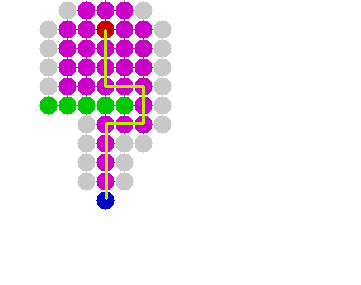
\includegraphics[width=0.5\textwidth]{img/screen_ue8_t2-1.png}\newpage
Plot for i=0:\\
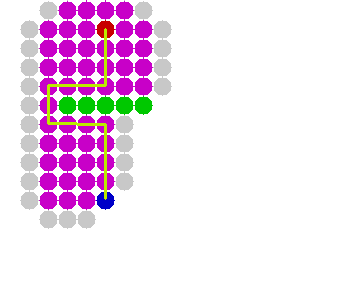
\includegraphics[width=0.5\textwidth]{img/screen_ue8_t2-2.png}\\
Plot for i=1:\\
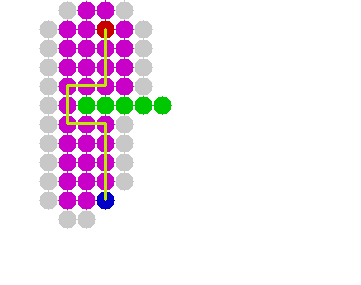
\includegraphics[width=0.5\textwidth]{img/screen_ue8_t2-3.png}